\documentclass[12pt,a4paper]{article}

\usepackage[utf8]{inputenc}
\usepackage[T1]{fontenc}
\usepackage{mathpazo}
\usepackage[margin=1.15in]{geometry}
\usepackage{setspace}
\usepackage{hyperref}
\usepackage{titlesec}
\usepackage{amsmath,amsthm,amssymb}
\usepackage{booktabs}
\usepackage{enumitem}
\usepackage{fancyhdr}
\usepackage{xcolor}
\usepackage{tcolorbox}
\usepackage{tikz}
\usepackage{array}
\usepackage{float}

\hypersetup{colorlinks=true, linkcolor=blue!70!black, citecolor=black, urlcolor=blue!70!black}

\titleformat{\section}{\large\bfseries}{\thesection}{0.7em}{}
\titleformat{\subsection}{\normalsize\bfseries}{\thesubsection}{0.7em}{}
\titleformat{\subsubsection}{\normalsize\itshape}{\thesubsubsection}{0.7em}{}

\newtheorem{definition}{Definition}[section]
\newtheorem{proposition}[definition]{Proposition}
\newtheorem{theorem}[definition]{Theorem}
\newtheorem{lemma}[definition]{Lemma}
\newtheorem{corollary}[definition]{Corollary}
\newtheorem{example}[definition]{Example}
\theoremstyle{remark}
\newtheorem{remark}[definition]{Remark}

\newcommand{\R}{\mathbb{R}}
\newcommand{\ones}{\mathbf{1}}
\newcommand{\x}{\mathbf{x}}
\DeclareMathOperator*{\argmax}{arg\,max}
\DeclareMathOperator{\Var}{Var}

\newtcolorbox{intuition}[1][]{colback=blue!3, colframe=blue!40!black,
  fonttitle=\bfseries, title={Intuition: #1}, sharp corners, boxrule=0.5pt}
\newtcolorbox{keyinsight}[1][]{colback=orange!5, colframe=orange!60!black,
  fonttitle=\bfseries, title={Key Structural Insight}, sharp corners, boxrule=0.5pt}
\newtcolorbox{prebisch}[1][]{colback=green!3, colframe=green!40!black,
  fonttitle=\bfseries, title={Prebisch Connection: #1}, sharp corners, boxrule=0.5pt}
\newtcolorbox{vizpanel}[1][]{colback=gray!4, colframe=gray!50!black,
  fonttitle=\bfseries, title={Visualization: #1}, sharp corners, boxrule=0.5pt}

\setlength{\parindent}{1.5em}
\onehalfspacing
\setlength{\headheight}{14pt}
\pagestyle{fancy}
\fancyhf{}
\fancyhead[L]{\small\itshape Chapter 14: Coalitions and Class Alliances}
\fancyhead[R]{\small\thepage}
\renewcommand{\headrulewidth}{0.4pt}

\title{\vspace{-1cm}\textbf{Chapter 14} \\[0.5em]
\LARGE Coalitions and Class Alliances \\[0.3em]
\large\textit{Who Allies with Whom to Change the Matrix}}
\author{}
\date{}

\begin{document}
\maketitle
\thispagestyle{fancy}

\begin{quote}
\textit{``N\~{a}o basta vincular de forma abstrata os modos de produ\c{c}\~{a}o e as formas de explora\c{c}\~{a}o \`{a}s fases do desenvolvimento capitalista. \'{E} necess\'{a}rio levar em conta as situa\c{c}\~{o}es em que se d\~{a}o as alian\c{c}as entre grupos e classes que atuam no sentido de manter uma dada estrutura de dom\'{i}nio ou de promover a sua transforma\c{c}\~{a}o.''}\\[0.3em]
\textnormal{[``It is not enough to link in abstract fashion the modes of production and forms of exploitation to the phases of capitalist development. It is necessary to take into account the situations in which the alliances between groups and classes act to maintain a given structure of domination or to promote its transformation.'']}\\
\hfill --- Fernando Henrique Cardoso and Enzo Faletto, \textit{Depend\^{e}ncia e Desenvolvimento na Am\'{e}rica Latina} (1969)
\end{quote}

\vspace{1em}

Chapter~13 showed how the weight matrix $W$ evolves through edge creation, destruction, and reweighting. But it treated the evolution as a stochastic process --- edges form or break according to surplus and proximity, as if the network rewires itself.

In practice, structural change is not automatic. It is \textit{political}. Agents form coalitions to change $W$ in their favor --- to strengthen the edges that increase their power and weaken the edges that benefit their rivals. Trade policy, labor regulation, land reform, media ownership, education access, border control --- all of these are instruments through which coalitions reshape the weight matrix.

This chapter introduces coalitions into the structural model. The key question: which coalitions form, and what do they do to $W$? The answer: a coalition $S \subseteq \{1, \ldots, N\}$ forms if its members collectively gain from the structural change they can enact. The gain is measured by $\Delta\boldsymbol{\pi}$: the change in the Perron eigenvector. A coalition is viable if every member gains power ($\Delta\pi_i > 0$ for all $i \in S$) and the coalition can implement the required $\Delta W$.


%% =====================================================================
\section{Coalitions as Network Designers}
\label{sec:coalitions}
%% =====================================================================

\subsection{The Coalition Problem}

\begin{definition}[Coalition]\label{def:coalition}
A \textbf{coalition} is a subset $S \subseteq \{1, \ldots, N\}$ of agents who jointly choose a structural change $\Delta W$ to maximize their collective power:
\begin{equation}\label{eq:coalition_objective}
\max_{\Delta W \in \mathcal{F}(S)} \sum_{i \in S} \pi_i(W + \Delta W),
\end{equation}
where $\mathcal{F}(S)$ is the \textbf{feasibility set}: the set of structural changes the coalition can implement given its current power.
\end{definition}

The feasibility set depends on what the coalition controls. An agent who controls a factory can rewire her production edges ($\Delta W^P$). An agent who controls a media outlet can rewire information edges ($\Delta W^I$). An agent who controls the state can use regulation, taxation, and subsidies to rewire multiple layers of $W$ simultaneously. The more powerful the coalition, the larger $\mathcal{F}(S)$.

\begin{proposition}[Power Determines Feasibility]\label{prop:feasibility}
The feasibility set of coalition $S$ is bounded by the coalition's current power:
\begin{equation}\label{eq:feasibility}
\mathcal{F}(S) = \left\{\Delta W : \|\Delta W\|_F \leq \phi\left(\sum_{i \in S} \pi_i(W)\right)\right\},
\end{equation}
where $\phi(\cdot)$ is an increasing function: coalitions with more power can implement larger structural changes. The rich get richer: the powerful can change the structure more, which makes them more powerful, which expands their feasibility set.
\end{proposition}

\begin{intuition}[The political Coase theorem fails]
Acemoglu (2003) asked: why don't societies always adopt efficient institutions? If the efficient structure benefits everyone (or at least generates a large enough surplus to compensate losers), why doesn't a grand coalition implement it?

The answer in this framework: the feasibility set depends on \textit{current} power. The coalition that would benefit from the efficient $W$ (the powerless majority) lacks the power to implement $\Delta W$. The coalition that has the power (the powerful minority) has no incentive to implement it --- the efficient $W$ would reduce their power. The political Coase theorem fails because the enforcement mechanism IS the current $W$, and $W$ is not neutral.
\end{intuition}


\subsection{The Payoff from a Coalition}

\begin{definition}[Coalition Payoff]\label{def:payoff}
The payoff to agent $i$ from joining coalition $S$ that implements $\Delta W_S$ is:
\begin{equation}\label{eq:payoff}
v_i(S) = x_i^*(W + \Delta W_S, \boldsymbol{\theta}^*_{W + \Delta W_S}) - x_i^*(W, \boldsymbol{\theta}^*_W).
\end{equation}
This includes both the enforcement effect (change in allocation at fixed preferences) and the formation effect (long-run change in allocation from preference adjustment):
\begin{equation}\label{eq:payoff_decomp}
v_i(S) = \underbrace{\Delta x_i^{\text{enf}}}_{\text{enforcement}} + \underbrace{\Delta x_i^{\text{form}}}_{\text{formation}} = E_i(\Delta W_S) + F_i(\Delta W_S).
\end{equation}
\end{definition}

\begin{proposition}[The Power Gain Approximation]\label{prop:power_gain}
In the LQ model, the enforcement payoff is approximately:
\begin{equation}\label{eq:power_gain}
E_i(\Delta W_S) \approx \frac{1}{\kappa}\Delta\pi_i(W, \Delta W_S),
\end{equation}
where $\Delta\pi_i = \pi_i(W + \Delta W_S) - \pi_i(W)$. The formation payoff is:
\begin{equation}\label{eq:formation_gain}
F_i(\Delta W_S) \approx \frac{\Psi}{\kappa}\Delta\pi_i(W, \Delta W_S),
\end{equation}
where $\Psi$ is the formation-to-enforcement ratio from Chapter~11. The total payoff:
\begin{equation}\label{eq:total_payoff}
v_i(S) \approx \frac{1 + \Psi}{\kappa}\Delta\pi_i.
\end{equation}
The payoff is proportional to the change in the Perron eigenvector, amplified by $(1 + \Psi)$.
\end{proposition}

\begin{keyinsight}
The coalition payoff is determined by $\Delta\boldsymbol{\pi}$: the change in the power vector. Every political conflict --- every trade war, labor dispute, media battle, land reform, nationalization --- is a fight over $\Delta\boldsymbol{\pi}$. The coalition that wins is the one that can implement the $\Delta W$ that shifts $\boldsymbol{\pi}$ in its favor.

The formation amplifier $(1 + \Psi)$ is crucial: when $\Psi > 0$, a structural change has long-run effects beyond the immediate power shift, because the new $W$ eventually changes preferences. A coalition that controls $W^I$ (media, education) benefits from the formation amplifier: not only does it gain power immediately, but it shapes the preferences of the next generation to \textit{accept} the new power structure. This is the deepest form of structural power: the power to make your power seem natural.
\end{keyinsight}


%% =====================================================================
\section{Which Coalitions Form?}
\label{sec:which}
%% =====================================================================

\subsection{Stability Concepts}

\begin{definition}[Stable Coalition Structure]\label{def:stable}
A partition of agents into coalitions $\mathcal{S} = \{S_1, S_2, \ldots, S_k\}$ is \textbf{stable} if:
\begin{enumerate}
\item \textbf{Internal stability}: No member of any coalition $S_m$ would prefer to defect (to leave $S_m$ and either join another coalition or stand alone). For all $i \in S_m$: $v_i(S_m) \geq v_i(S_m \setminus \{i\})$ and $v_i(S_m) \geq v_i(\{i\})$.
\item \textbf{External stability}: No coalition $S_m$ would accept a new member from outside. For all $j \notin S_m$: if $j$ wants to join $S_m$, then at least one existing member of $S_m$ would be made worse off.
\item \textbf{Coalition rationality}: Each coalition implements the $\Delta W_S$ that maximizes its collective payoff given the other coalitions' actions.
\end{enumerate}
\end{definition}

\begin{theorem}[Coalition Formation Theorem]\label{thm:formation}
In the structural model with $N$ agents and LQ payoffs:
\begin{enumerate}
\item At least one stable coalition structure exists (under compact feasibility sets and continuous payoffs).
\item The grand coalition $S = \{1, \ldots, N\}$ is stable if and only if the efficient $W^*$ is in $\mathcal{F}(\{1, \ldots, N\})$ and the surplus from efficiency can compensate every agent for her power loss. This requires side payments --- which may not be credible if the current $W$ is the enforcement mechanism (Acemoglu's point).
\item In general, the stable partition involves 2--3 coalitions that balance each other's power.
\end{enumerate}
\end{theorem}

\begin{proof}[Proof sketch]
(1) The existence follows from the theory of coalition-proof Nash equilibria (Bernheim, Peleg, and Whinston, 1987) adapted to the structural game. (2) The grand coalition implements $W^{CE} = \frac{1}{N}\ones\ones'$ (the efficient structure). The surplus is maximized. But agent $i$ with $\pi_i > 1/N$ loses power, so she must be compensated by a transfer. The transfer must be credible --- but credible transfers require an enforcement mechanism, and the enforcement mechanism IS the current $W$, which the grand coalition proposes to change. (3) With 2--3 coalitions, each has enough power to implement local $\Delta W$ but not enough to achieve the grand coalition's global restructuring.
\end{proof}


\subsection{The Class Alliance as a Coalition}

\begin{definition}[Class Alliance]\label{def:class_alliance}
A \textbf{class alliance} is a coalition formed between agents from different structural positions (blocks of $W$) who share a common interest in a specific $\Delta W$. The alliance is stable if all members gain from the structural change, despite occupying different positions in the current structure.
\end{definition}

\begin{example}[Four Class Alliances in Latin America]\label{ex:four_alliances}
Four agents: Foreign Capital ($F$), Domestic Bourgeoisie ($B$), Middle Class ($M$), Workers ($W$). Current power: $\boldsymbol{\pi} = (0.35, 0.30, 0.20, 0.15)$.

\textbf{Alliance 1: Oligarchic-Export ($\{F, B\}$).} Foreign capital and domestic landowners/miners export raw materials. They strengthen $W^P_{\text{FB}}$ (supply chain links) and $W^I_{\text{FB}}$ (shared business culture). The structural change reinforces the export enclave:
\begin{equation}
\Delta\boldsymbol{\pi} \approx (+0.05, +0.03, -0.04, -0.04).
\end{equation}
$F$ and $B$ gain; $M$ and $W$ lose. The enclave deepens.

\textbf{Alliance 2: National-Populist ($\{B, M, W\}$).} Domestic bourgeoisie, middle class, and workers unite against foreign capital. They implement ISI: tariffs weaken $W^P_{\text{F,domestic}}$ (fewer imported inputs) and strengthen $W^P_{\text{domestic}}$ (local supply chains). New domestic $W^I$ channels (national media, public education):
\begin{equation}
\Delta\boldsymbol{\pi} \approx (-0.12, +0.05, +0.04, +0.03).
\end{equation}
$F$ loses massively; all domestic classes gain. Per\'{o}n's Argentina, Vargas's Brazil, the MNR in Bolivia.

\textbf{Alliance 3: Techno-Bureaucratic ($\{F, B, M\}$ excluding $W$).} Post-coup modernization. Foreign capital, domestic bourgeoisie, and the technical middle class ally to implement ``efficient'' structural adjustment. They strengthen $W^P_{\text{FB}}$ and $W^P_{\text{BM}}$ while weakening labor protections ($W^U_{WM}$ and $W^I_{WM}$ edges severed):
\begin{equation}
\Delta\boldsymbol{\pi} \approx (+0.03, +0.04, +0.02, -0.09).
\end{equation}
Workers bear all the cost. Brazil post-1964, Chile post-1973, Bolivia 1985.

\textbf{Alliance 4: Left-Populist ($\{M, W\}$ sometimes $+ B$).} Middle class and workers unite, sometimes pulling in the domestic bourgeoisie against foreign capital. They nationalize key sectors ($\Delta W^P$: gas/mining edges redirect from $F$ to state), expand public $W^I$ (state media, education reform), and strengthen labor linkages ($W^U_{MW}$):
\begin{equation}
\Delta\boldsymbol{\pi} \approx (-0.10, -0.02, +0.05, +0.07).
\end{equation}
$F$ loses most; $W$ gains most. Evo Morales's Bolivia, Ch\'{a}vez's Venezuela.
\end{example}

\begin{vizpanel}{Four alliances, four $\Delta\boldsymbol{\pi}$ vectors}
\begin{center}
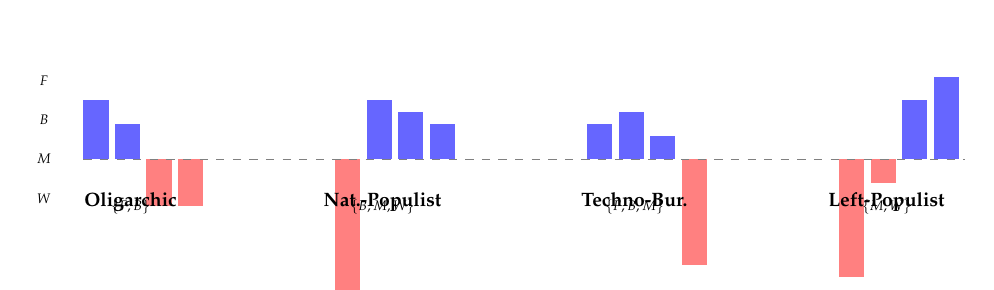
\begin{tikzpicture}[scale=1]
\def\bw{0.4}

%% Alliance 1: Oligarchic
\foreach \k/\val/\sgn in {1/0.05/1,2/0.03/1,3/-0.04/-1,4/-0.04/-1} {
  \pgfmathparse{\sgn > 0 ? "blue!60" : "red!50"}
  \edef\col{\pgfmathresult}
  \fill[\col] ({(\k-1)*\bw}, 0) rectangle ({(\k-1)*\bw+\bw*0.8}, {\val*15});
}
\node[font=\scriptsize\bfseries, below] at ({1.5*\bw}, -0.3) {Oligarchic};
\node[font=\tiny] at ({1.5*\bw}, -0.6) {$\{F,B\}$};

%% Alliance 2: National-Populist
\begin{scope}[xshift=3.2cm]
\foreach \k/\val in {1/-0.12,2/0.05,3/0.04,4/0.03} {
  \pgfmathparse{\val > 0 ? "blue!60" : "red!50"}
  \edef\col{\pgfmathresult}
  \fill[\col] ({(\k-1)*\bw}, 0) rectangle ({(\k-1)*\bw+\bw*0.8}, {\val*15});
}
\node[font=\scriptsize\bfseries, below] at ({1.5*\bw}, -0.3) {Nat.-Populist};
\node[font=\tiny] at ({1.5*\bw}, -0.6) {$\{B,M,W\}$};
\end{scope}

%% Alliance 3: Techno-Bureaucratic
\begin{scope}[xshift=6.4cm]
\foreach \k/\val in {1/0.03,2/0.04,3/0.02,4/-0.09} {
  \pgfmathparse{\val > 0 ? "blue!60" : "red!50"}
  \edef\col{\pgfmathresult}
  \fill[\col] ({(\k-1)*\bw}, 0) rectangle ({(\k-1)*\bw+\bw*0.8}, {\val*15});
}
\node[font=\scriptsize\bfseries, below] at ({1.5*\bw}, -0.3) {Techno-Bur.};
\node[font=\tiny] at ({1.5*\bw}, -0.6) {$\{F,B,M\}$};
\end{scope}

%% Alliance 4: Left-Populist
\begin{scope}[xshift=9.6cm]
\foreach \k/\val in {1/-0.10,2/-0.02,3/0.05,4/0.07} {
  \pgfmathparse{\val > 0 ? "blue!60" : "red!50"}
  \edef\col{\pgfmathresult}
  \fill[\col] ({(\k-1)*\bw}, 0) rectangle ({(\k-1)*\bw+\bw*0.8}, {\val*15});
}
\node[font=\scriptsize\bfseries, below] at ({1.5*\bw}, -0.3) {Left-Populist};
\node[font=\tiny] at ({1.5*\bw}, -0.6) {$\{M,W\}$};
\end{scope}

%% Legend
\draw[gray, dashed] (0, 0) -- (11.2, 0);
\node[font=\tiny] at (-0.5, 1.0) {$F$};
\node[font=\tiny] at (-0.5, 0.5) {$B$};
\node[font=\tiny] at (-0.5, 0.0) {$M$};
\node[font=\tiny] at (-0.5, -0.5) {$W$};
\end{tikzpicture}
\end{center}
\vspace{-0.5em}
\small Four bars per alliance: $\Delta\pi_F$, $\Delta\pi_B$, $\Delta\pi_M$, $\Delta\pi_W$. Blue bars (above zero): the agent gains power. Red bars (below): she loses. Each alliance is defined by who gains and who pays. The bars are $\Delta\boldsymbol{\pi}$ --- the object that every political conflict is about.
\end{vizpanel}


%% =====================================================================
\section{The Stability of Alliances}
\label{sec:stability}
%% =====================================================================

\subsection{When Alliances Hold}

\begin{proposition}[Alliance Stability Conditions]\label{prop:alliance_stability}
Alliance $S$ is internally stable (no member wants to defect) if and only if:
\begin{equation}\label{eq:internal}
\Delta\pi_i(W, \Delta W_S) > 0 \quad \text{for all } i \in S,
\end{equation}
AND no member can achieve a higher $\Delta\pi_i$ by defecting to a rival alliance $S'$:
\begin{equation}\label{eq:no_defect}
\Delta\pi_i(W, \Delta W_S) \geq \Delta\pi_i(W, \Delta W_{S' \cup \{i\}}) \quad \text{for all feasible } S'.
\end{equation}
\end{proposition}

\begin{example}[Why the National-Populist Alliance Breaks]\label{ex:breaks}
Consider Alliance~2 ($\{B, M, W\}$). Initially stable: all three domestic classes gain from ISI. But as ISI succeeds, the domestic bourgeoisie grows --- her $\pi_B$ increases. At some threshold, she can earn a higher $\Delta\pi_B$ by switching to Alliance~3 ($\{F, B, M\}$): partnering with foreign capital to ``open'' the economy.

The switch occurs when:
\begin{equation}\label{eq:switch}
\Delta\pi_B(\Delta W_{\{F,B,M\}}) > \Delta\pi_B(\Delta W_{\{B,M,W\}}).
\end{equation}

In words: when the domestic bourgeoisie is strong enough that partnering with foreign capital (and cutting out workers) yields a higher power gain than continuing the national-populist alliance. This is the transition from ISI populism to techno-bureaucratic modernization --- the story of Brazil 1964, Argentina 1976, Chile 1973.

\begin{center}
\begin{tabular}{lccc}
\toprule
Phase & Alliance & $\pi_B$ & $\Delta\pi_B$ from best alliance \\
\midrule
Early ISI & $\{B, M, W\}$ & 0.20 & $+0.05$ \\
Mature ISI & $\{B, M, W\}$ & 0.30 & $+0.03$ (diminishing) \\
Post-ISI crisis & Switch to $\{F, B, M\}$ & 0.30 & $+0.04$ \\
\bottomrule
\end{tabular}
\end{center}

The alliance breaks because its own success changes the power structure, which changes the payoffs, which changes the optimal alliance. The matrix $W$ evolved (Chapter~13), and the evolution shifted the coalition incentives.
\end{example}


\subsection{When Alliances Cycle}

\begin{theorem}[Alliance Cycling]\label{thm:cycling}
In the co-evolutionary system with coalition formation, the following cycle can occur:
\begin{enumerate}
\item Phase~1: National-populist alliance ($\{B, M, W\}$) implements ISI. $\pi_B$ rises. Domestic $\Gamma$ increases.
\item Phase~2: $B$ defects to techno-bureaucratic alliance ($\{F, B, M\}$). Liberalization. $\pi_W$ falls. $W^I$ becomes more center-dominated.
\item Phase~3: Workers and middle class form left-populist alliance ($\{M, W\}$, sometimes $+B$). Nationalization. $\pi_F$ falls. Domestic $\Gamma$ increases again.
\item Phase~4: Resource rents create corruption/inefficiency. $B$ defects again to $\{F, B\}$ or $\{F, B, M\}$. Return to Phase~2.
\end{enumerate}
The cycle is the \textbf{Latin American pendulum}: ISI $\to$ liberalization $\to$ populism $\to$ liberalization $\to \cdots$
\end{theorem}

\begin{proof}[Proof sketch]
Each phase changes $W$, which changes $\boldsymbol{\pi}$, which changes the coalition payoffs $\Delta\pi_i(S)$, which destabilizes the current alliance and triggers a switch. The cycle is sustained because no single structural equilibrium satisfies all agents simultaneously: the efficient $W$ requires the grand coalition, but the grand coalition requires credible commitment, which requires the enforcement mechanism that the coalition proposes to change.
\end{proof}

\begin{prebisch}[The Latin American pendulum]
The cycling theorem formalizes what economic historians of Latin America have observed for a century: the oscillation between inward-oriented and outward-oriented development strategies, between populist inclusion and technocratic exclusion, between nationalization and liberalization.

The standard explanation is ``policy failure'': populism leads to fiscal crisis, which triggers liberalization, which leads to inequality, which triggers populism. This explanation blames the cycle on bad policy.

The structural explanation is different: the cycle is endogenous to the co-evolutionary system. Each alliance changes $W$ in a way that eventually destabilizes itself. ISI strengthens the bourgeoisie, who then defects. Liberalization weakens workers, who then rebel. Nationalization creates rents, which corrupt the coalition. The cycle is not a sequence of mistakes. It is the dynamics of a system that has no stable grand coalition because the enforcement mechanism is the object being contested.

Bolivia's cycle: MNR revolution (1952, Alliance~2) $\to$ military/technocratic rule (1964, Alliance~3) $\to$ democratic opening and structural adjustment (1985, Alliance~3 variant) $\to$ resource nationalism (2006, Alliance~4) $\to$ political crisis (2019, unstable). Each transition is a coalition switch driven by $\Delta\boldsymbol{\pi}$.
\end{prebisch}


%% =====================================================================
\section{The Structural Power Game}
\label{sec:game}
%% =====================================================================

\subsection{Formalization}

\begin{definition}[The Structural Power Game]\label{def:game}
The \textbf{structural power game} $\mathcal{G} = (N, \{A_i\}, \{v_i\}, W)$ is defined by:
\begin{itemize}
\item $N$ players (agents or classes).
\item Action set $A_i$: the set of coalitions agent $i$ can join.
\item Payoff $v_i(S) = \frac{1+\Psi}{\kappa}\Delta\pi_i(W, \Delta W_S)$: the allocation change from the coalition's structural policy.
\item The current weight matrix $W$, which determines both the payoffs and the feasibility sets.
\end{itemize}
\end{definition}

\begin{proposition}[Properties of the Structural Power Game]\label{prop:game_properties}
\begin{enumerate}
\item The game is \textbf{not zero-sum}: the efficient structural change ($W \to W^{CE}$) increases total welfare. But the game is \textbf{redistributive}: any $\Delta W$ that increases $\pi_i$ for some $i$ decreases $\pi_j$ for some $j$ (since $\sum_i \pi_i = 1$).
\item The game is \textbf{not superadditive}: the grand coalition may not yield the highest payoff for every agent, because the efficient $W$ reduces the power of currently powerful agents.
\item The game is \textbf{path-dependent}: the current $W$ determines the feasibility sets, which determine which coalitions can form, which determines the next $W$. History matters.
\item The \textbf{core} of the game (the set of allocations that no coalition can improve upon) may be empty when $W$ is highly asymmetric (concentrated power).
\end{enumerate}
\end{proposition}


\subsection{Equilibrium Alliance Structures}

\begin{theorem}[Equilibrium Characterization]\label{thm:equilibrium}
In the structural power game with $N = 4$ (Foreign Capital, Domestic Bourgeoisie, Middle Class, Workers):
\begin{enumerate}
\item If $\pi_F > 0.4$ (foreign capital dominant): the stable alliance is $\{F, B\}$ (oligarchic-export). Workers and middle class cannot form a winning counter-coalition because $\mathcal{F}(\{M, W\})$ is too small.
\item If $\pi_B > \pi_F$ and $\pi_B + \pi_M + \pi_W > 0.5$ (domestic bourgeoisie strong, collective domestic power exceeds foreign): the stable alliance is $\{B, M, W\}$ (national-populist).
\item If $\pi_B + \pi_F > \pi_M + \pi_W$ and $\pi_W < 0.15$ (workers very weak): the stable alliance is $\{F, B, M\}$ (techno-bureaucratic).
\item If $\pi_M + \pi_W > \pi_F + \pi_B$ (domestic non-elite majority is powerful enough): the stable alliance is $\{M, W\}$ or $\{B, M, W\}$ (left-populist or national-populist).
\end{enumerate}
\end{theorem}

\begin{vizpanel}{Alliance stability regions in the $(\pi_F, \pi_W)$ plane}
\begin{center}
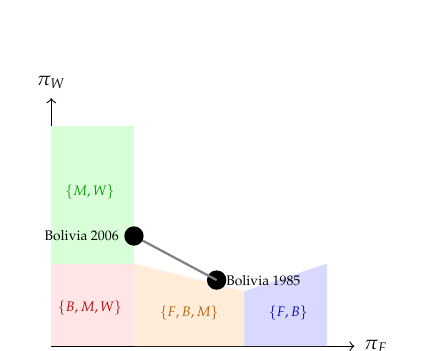
\begin{tikzpicture}[scale=7]
%% Axes
\draw[->] (0,0) -- (0.55,0) node[right, font=\scriptsize] {$\pi_F$};
\draw[->] (0,0) -- (0,0.45) node[above, font=\scriptsize] {$\pi_W$};

%% Regions (approximate)
\fill[blue!15] (0.35,0) -- (0.5,0) -- (0.5,0.15) -- (0.35,0.10) -- cycle;
\node[font=\tiny, blue!70!black] at (0.43, 0.06) {$\{F,B\}$};

\fill[green!15] (0,0.15) -- (0.15,0.15) -- (0.15,0.40) -- (0,0.40) -- cycle;
\node[font=\tiny, green!60!black] at (0.07, 0.28) {$\{M,W\}$};

\fill[orange!15] (0.15,0) -- (0.35,0) -- (0.35,0.10) -- (0.15,0.15) -- cycle;
\node[font=\tiny, orange!70!black] at (0.25, 0.06) {$\{F,B,M\}$};

\fill[red!10] (0.0,0.0) -- (0.15,0.0) -- (0.15,0.15) -- (0.0,0.15) -- cycle;
\node[font=\tiny, red!70!black] at (0.07, 0.07) {$\{B,M,W\}$};

%% Bolivia trajectory
\fill (0.30, 0.12) circle (0.5pt);
\node[font=\tiny, right] at (0.30, 0.12) {Bolivia 1985};
\draw[->, thick, gray] (0.30, 0.12) -- (0.15, 0.20);
\fill (0.15, 0.20) circle (0.5pt);
\node[font=\tiny, left] at (0.14, 0.20) {Bolivia 2006};
\end{tikzpicture}
\end{center}
\vspace{-0.5em}
\small Each region corresponds to a stable alliance structure, determined by the power distribution $(\pi_F, \pi_W)$ (with $\pi_B$ and $\pi_M$ filling the remainder). Bolivia moved from the techno-bureaucratic region (1985: $\pi_F$ high, $\pi_W$ low) to the left-populist region (2006: $\pi_F$ lower, $\pi_W$ higher). The arrow is one step of the Latin American pendulum.
\end{vizpanel}


%% =====================================================================
\section{Structural Policy as Coalition Output}
\label{sec:policy}
%% =====================================================================

Every structural policy is a specific $\Delta W$ chosen by a specific coalition. The table of policies from Chapter~10 (transfers, structural policy, information policy) can now be mapped to coalitions:

\begin{proposition}[Policy as Coalition Output]\label{prop:policy_coalition}
\begin{center}
\begin{tabular}{llll}
\toprule
\textbf{Policy} & \textbf{$\Delta W$} & \textbf{Typical coalition} & \textbf{$\Delta\boldsymbol{\pi}$ pattern} \\
\midrule
Trade liberalization & $W^P_{\text{domestic}} \downarrow$, $W^P_{\text{global}} \uparrow$ & $\{F, B\}$ or $\{F, B, M\}$ & $\pi_F \uparrow$, $\pi_W \downarrow$ \\
ISI / industrial policy & $W^P_{\text{domestic}} \uparrow$, $W^P_{\text{global}} \downarrow$ & $\{B, M, W\}$ & $\pi_B \uparrow$, $\pi_F \downarrow$ \\
Nationalization & $W^P_{\text{F}} \to W^P_{\text{state}}$ & $\{M, W\}$ or $\{B, M, W\}$ & $\pi_F \downarrow$, $\pi_M \uparrow$ \\
Land reform & $W^P_{\text{landlord}} \to W^P_{\text{farmer}}$ & $\{M, W\}$ & $\pi_{\text{landlord}} \downarrow$ \\
Media regulation & $\Delta W^I$ (de-concentrate) & $\{M, W\}$ or $\{B, M, W\}$ & $N_{\text{eff}} \uparrow$ \\
Education expansion & $\Delta W^I$ (cross-block edges) & Variable & $\Psi$-amplified \\
Cash transfers & $\Delta\boldsymbol{\omega}$ (not $\Delta W$) & Any & $\Delta\boldsymbol{\pi} = 0$ \\
\bottomrule
\end{tabular}
\end{center}
Note: cash transfers (last row) do not change $W$ and therefore do not change $\boldsymbol{\pi}$. This is the Transfer Trap from Chapter~2, now with a political explanation: every coalition can agree on transfers (they don't threaten anyone's structural power), but no coalition will implement the $\Delta W$ that reduces its own $\boldsymbol{\pi}$.
\end{proposition}


%% =====================================================================
\section{Summary}
\label{sec:summary}
%% =====================================================================

\begin{enumerate}
\item \textbf{Coalitions} are subsets of agents who jointly choose $\Delta W$ to maximize their collective power. The feasibility set $\mathcal{F}(S)$ depends on current power: the powerful can change more.

\item The \textbf{coalition payoff} is $v_i(S) \approx \frac{1+\Psi}{\kappa}\Delta\pi_i$: proportional to the change in the Perron eigenvector, amplified by the formation multiplier.

\item \textbf{Four Latin American alliances}: oligarchic-export $\{F,B\}$, national-populist $\{B,M,W\}$, techno-bureaucratic $\{F,B,M\}$, left-populist $\{M,W\}$. Each implements a different $\Delta W$ with a different $\Delta\boldsymbol{\pi}$.

\item \textbf{Alliance cycling}: ISI strengthens $B$, who defects $\to$ liberalization weakens $W$, who rebels $\to$ populism $\to$ crisis $\to$ repeat. The cycle is endogenous: each alliance's success changes the power structure that destabilizes it.

\item The \textbf{political Coase theorem fails} because the enforcement mechanism IS the current $W$. The grand coalition requires credible commitment, which requires an institution that the coalition proposes to change.

\item \textbf{Cash transfers} are the one policy every coalition can agree on, precisely because they change $\boldsymbol{\omega}$ but not $\boldsymbol{\pi}$.
\end{enumerate}


%% =====================================================================
\section{Exercises}
\label{sec:exercises}
%% =====================================================================

\begin{enumerate}[label=\textbf{14.\arabic*}, leftmargin=3em]

\item \textbf{Coalition payoffs.} For $N = 4$ with $\boldsymbol{\pi} = (0.35, 0.30, 0.20, 0.15)$ and $\kappa = 0.5$:
\begin{enumerate}
\item Compute the current bargaining allocation $\x^*$.
\item Coalition $\{3, 4\}$ (workers and middle class) implements $\Delta W$ that shifts $\boldsymbol{\pi}$ to $(0.25, 0.25, 0.25, 0.25)$. Compute $v_3(\{3,4\})$ and $v_4(\{3,4\})$. Are both positive?
\item Can $\{3, 4\}$ implement this $\Delta W$? Check feasibility: $\|\Delta W\|_F \leq \phi(\pi_3 + \pi_4) = \phi(0.35)$.
\item Agent 2 considers defecting from $\{1, 2\}$ to $\{2, 3, 4\}$. Compute $\Delta\pi_2$ under both coalitions. Which does she prefer?
\end{enumerate}

\item \textbf{Alliance stability.} For Example~\ref{ex:four_alliances}: verify that each alliance is internally stable (all members gain) and identify the conditions under which each breaks.

\item \textbf{The Latin American pendulum.} Simulate the cycling theorem for 8 periods. Start with Alliance~2 ($\{B,M,W\}$). At each period: (a) compute the coalition's $\Delta W$ and new $\boldsymbol{\pi}$, (b) check whether any member wants to defect, (c) if so, form the new alliance. Plot $\boldsymbol{\pi}_t$ over time. Does it cycle?

\item \textbf{Bolivia 1952--2019.} Map Bolivia's political history to the four-alliance framework:
\begin{enumerate}
\item MNR Revolution (1952): which alliance? What $\Delta W$?
\item Military governments (1964--1982): alliance switch to what?
\item Structural adjustment (1985): which alliance implements the NEP?
\item Evo Morales (2006): alliance switch to what? What $\Delta W^P$ (nationalization)?
\item Political crisis (2019): alliance breakdown. Which conditions from Proposition~\ref{prop:alliance_stability} failed?
\end{enumerate}

\item \textbf{Why cash transfers are universal.} Show formally that $\Delta\boldsymbol{\pi}(\Delta\boldsymbol{\omega}) = 0$: transfers do not change the Perron eigenvector. Explain why this makes transfers the \textit{least controversial} policy tool: no agent's structural power is threatened. Then explain why this makes transfers the \textit{least effective} tool for structural change.

\item \textbf{The formation amplifier in politics.} Compare two alliances with the same $\Delta\boldsymbol{\pi}$ but different $\Psi$:
\begin{enumerate}
\item Alliance A controls $W^P$ (production policy): $\Psi_A \approx 1$.
\item Alliance B controls $W^I$ (media, education): $\Psi_B \approx 3$.
\item Compute the total payoff $v_i = \frac{1+\Psi}{\kappa}\Delta\pi_i$ for each. Which alliance is more valuable to its members?
\item Which type of alliance is harder to form? (Hint: controlling $W^I$ may require controlling the state first, which requires power, which requires an alliance\ldots)
\end{enumerate}

\item \textbf{Empty core.} Construct a 3-agent structural power game where the core is empty: for every coalition structure, some coalition can profitably deviate. Show that this implies cycling. What property of $W$ produces an empty core? (Hint: extreme asymmetry.)
\end{enumerate}


%% =====================================================================
\newpage
\section*{Mathematical Appendices}
\addcontentsline{toc}{section}{Mathematical Appendices}
%% =====================================================================


\subsection*{Appendix 14A: Cooperative Game Theory for Structural Change}
\addcontentsline{toc}{subsection}{Appendix 14A: Cooperative Game Theory}
\label{app:cooperative}

\paragraph{The transferable-utility game.} A TU game is $(N, v)$ where $v: 2^N \to \R$ assigns a value to each coalition. The \textbf{core} is the set of payoff vectors $\x$ with $\sum_{i \in S} x_i \geq v(S)$ for all $S$ and $\sum_i x_i = v(N)$. The core is non-empty if and only if the game is balanced (Bondareva-Shapley theorem).

\paragraph{Application to structural change.} The structural power game is NOT a standard TU game because: (1) the value of a coalition depends on the current $W$ (state-dependent), (2) the feasibility set depends on power (endogenous constraints), and (3) the formation amplifier $(1+\Psi)$ makes payoffs time-dependent (they include long-run preference effects). Nevertheless, the core concept provides useful predictions about which alliance structures are stable.

\paragraph{The Shapley value.} The Shapley value $\phi_i = \sum_{S \subseteq N \setminus \{i\}} \frac{|S|!(N-|S|-1)!}{N!}[v(S \cup \{i\}) - v(S)]$ gives each agent her average marginal contribution across all possible coalitions. In the structural power game, $\phi_i$ measures agent $i$'s ``structural leverage'' --- how much she improves any coalition she joins. Agents with high Shapley values are the ``kingmakers'' whose alliance decisions determine the political equilibrium.


\subsection*{Appendix 14B: Sensitivity of $\boldsymbol{\pi}$ to $\Delta W$}
\addcontentsline{toc}{subsection}{Appendix 14B: Sensitivity of $\boldsymbol{\pi}$}
\label{app:sensitivity}

\paragraph{First-order perturbation.} From Chapter~8 (Appendix 8B), the first-order change in the Perron eigenvector from a perturbation $\Delta W$:
\begin{equation}
\Delta\pi_i \approx \sum_{k=2}^N \frac{1}{1 - \lambda_k} u_{ki} \left(\mathbf{u}_k' \Delta W \mathbf{v}_1\right),
\end{equation}
where $\lambda_k$ are the eigenvalues of $W$, $\mathbf{u}_k$ are left eigenvectors, and $\mathbf{v}_1 = \ones$ is the right Perron eigenvector.

\paragraph{Implication for coalitions.} The ``cheapest'' $\Delta\boldsymbol{\pi}$ is achieved by perturbing $W$ in the direction of the most sensitive eigenvector (the one with $\lambda_k$ closest to 1). When the spectral gap $\Gamma$ is small, small perturbations produce large changes in $\boldsymbol{\pi}$ --- meaning that coalitions need less power to achieve large structural effects. Fragmented economies ($\Gamma \approx 0$) are politically unstable because small coalitions can tip the power structure.


%% =====================================================================
\subsection*{Structuralist Case Study: Cardoso and Faletto's Class Alliances}
\addcontentsline{toc}{subsection}{Structuralist Case Study: Cardoso and Faletto (1969)}
%% =====================================================================

This is Cardoso and Faletto's second appearance in the book. In Chapter~10, their ``situations of dependency'' were mapped to network topologies --- different configurations of $(W^P, W^U, W^I)$ producing different structural equilibria. Here, their analysis of class alliances provides the political mechanism that determines \textit{which} topology obtains.

The distinctive contribution of \textit{Depend\^{e}ncia e Desenvolvimento} was the insistence that economic outcomes cannot be read off from structural position alone. Two countries with identical $W^P$ (same export structure, same degree of foreign penetration) can have radically different development trajectories because the \textit{class alliances} differ. Brazil's post-1964 trajectory (techno-bureaucratic $\{F, B, M\}$) and Argentina's post-1946 trajectory (national-populist $\{B, M, W\}$) cannot be explained by their trade structures (both were semi-industrialized primary exporters). They can be explained by the alliances.

\textbf{Part 1: The alliance determines $\Delta W$, not vice versa.} The standard structuralist analysis (Prebisch, Furtado, Pinto) starts from $W$ and derives the allocation. Cardoso and Faletto reversed the causation for the political layer: the alliance determines which $\Delta W$ is implemented, and therefore which $W_{t+1}$ obtains. Different alliances produce different structural changes even from the same starting $W$. In this chapter's notation: the coalition $S$ is the independent variable; $\Delta W_S$ is the dependent variable. Political agency enters the model through coalition formation, not through the network evolution equation's stochastic mechanics.

\textbf{Part 2: Alliances are constrained by but not determined by structure.} Cardoso and Faletto rejected mechanical determinism: the structure constrains which alliances are feasible (through $\mathcal{F}(S)$) but does not uniquely determine which alliance forms. In the same structural situation, different political choices can lead to different alliances (Brazil chose techno-bureaucratic in 1964; Peru chose military-populist in 1968; Chile chose democratic-socialist in 1970 --- all from similar structural positions). The model of this chapter captures this through multiple equilibria in the structural power game (Theorem~\ref{thm:equilibrium}): the stable alliance is not unique, and the selection among equilibria depends on political contingency.

\textbf{Part 3: The alliance IS the development strategy.} The deepest insight: Cardoso and Faletto argued that ``the development strategy'' is not chosen by a benevolent planner who evaluates alternatives on efficiency grounds. The strategy is the $\Delta W$ that the winning coalition implements to maximize its collective $\boldsymbol{\pi}$. ISI was not chosen because it was ``efficient'' --- it was chosen because it was the structural policy preferred by the $\{B, M, W\}$ coalition. Liberalization was not chosen because it was ``efficient'' --- it was chosen because it was preferred by the $\{F, B, M\}$ coalition. The policy debate between ISI and liberalization is, in this framework, a debate between coalitions with different $\Delta\boldsymbol{\pi}$ interests disguised as a debate about economic theory.

\begin{center}
\begin{tabular}{lll}
\toprule
\textbf{Cardoso \& Faletto's argument} & \textbf{Formal object} & \textbf{This chapter} \\
\midrule
Class alliances shape the structure & Coalition $S$ chooses $\Delta W_S$ & Def.~\ref{def:coalition} \\
Alliances are constrained by structure & $\mathcal{F}(S)$ depends on $\sum_{i \in S} \pi_i$ & Prop.~\ref{prop:feasibility} \\
Same structure, different alliances & Multiple equilibria in the power game & Thm.~\ref{thm:equilibrium} \\
Development strategy = coalition output & $\Delta W$ maximizes coalition $\sum \Delta\pi_i$ & Def.~\ref{def:payoff} \\
Pendulum: ISI $\to$ liberalization $\to$ & Alliance cycling from co-evolutionary dynamics & Thm.~\ref{thm:cycling} \\
Political Coase theorem fails & Enforcement mechanism IS the current $W$ & Prop.~\ref{prop:feasibility} \\
\bottomrule
\end{tabular}
\end{center}

Cardoso became President and implemented the Plano Real (monetary stabilization) and a broadly liberal economic program --- closer to Alliance~3 ($\{F, B, M\}$) than to the national-populist program his academic work had analyzed. Whether this proves or disproves the model is an exercise the reader should not skip (Exercise~14.4 is related but more general). What the model predicts is that the alliance a politician joins depends on the current $\boldsymbol{\pi}$, not on the politician's academic publications. When $\boldsymbol{\pi}$ changes, the optimal alliance changes, and the development strategy changes with it.


%% =====================================================================
\subsection*{Further Reading}
\addcontentsline{toc}{subsection}{Further Reading}
%% =====================================================================

\textbf{Coalition formation:} Bernheim, Peleg, and Whinston (1987), ``Coalition-Proof Nash Equilibria,'' \textit{JET}. Ray and Vohra (1997), ``Equilibrium Binding Agreements,'' \textit{JET}. Acemoglu, Egorov, and Sonin (2012), ``Dynamics and Stability of Constitutions, Coalitions, and Clubs,'' \textit{AER}.

\textbf{The political economy of development:} Acemoglu (2003), ``Why Not a Political Coase Theorem?'' \textit{JCE}. Acemoglu and Robinson (2006), \textit{Economic Origins of Dictatorship and Democracy}. Bardhan (2005), \textit{Scarcity, Conflicts, and Cooperation}.

\textbf{Class alliances in Latin America:} Cardoso and Faletto (1969), \textit{Depend\^{e}ncia e Desenvolvimento}, especially Chapters~4--6 (the empirical alliance analysis for Argentina, Brazil, Chile, Mexico). O'Donnell (1973), \textit{Modernization and Bureaucratic-Authoritarianism}, for the formalization of the transition from populist to bureaucratic-authoritarian regimes. Collier and Collier (1991), \textit{Shaping the Political Arena}, for the long-run consequences of labor incorporation strategies.

\textbf{Bolivia's political economy:} Klein (2011), \textit{A Concise History of Bolivia}, Chapters~8--12. Dunkerley (1984), \textit{Rebellion in the Veins}. Webber (2011), \textit{From Rebellion to Reform in Bolivia}.


\end{document}
